% !TEX spellcheck=en_US
\documentclass[a4paper]{article}
\usepackage[american]{babel}
\usepackage[T1]{fontenc}
\usepackage[utf8]{inputenc}
\usepackage{graphicx}
\usepackage[table]{xcolor}
\usepackage{caption}
\usepackage{subcaption}
\usepackage{csquotes}
\usepackage{hyperref}
\usepackage[acronym]{glossaries}
\usepackage{amsmath}
\usepackage{amssymb}
\usepackage{amsthm}
\usepackage{mathtools}
\usepackage[backend=biber,style=phys]{biblatex}

\addbibresource{bibliography.bib}

\DeclareMathOperator\rank{rank}
\DeclareMathOperator\Span{Span}
\DeclareMathOperator\Col{Col}
\DeclareMathOperator\Row{Row}
\DeclareMathOperator\Null{Null}
\DeclareMathOperator\adj{adj}
\DeclareMathOperator\trace{tr}
\DeclareMathOperator\diag{diag}
\DeclareMathOperator\Hom{Hom}
\DeclareMathOperator\Floor{floor}
\DeclareMathOperator\Ceil{ceil}

\DeclarePairedDelimiter{\abs}{\lvert}{\rvert}
\DeclarePairedDelimiter{\norm}{\lVert}{\rVert}
\DeclarePairedDelimiter{\ceil}{\lceil}{\rceil}
\DeclarePairedDelimiter{\floor}{\lfloor}{\rfloor}

\newcommand*{\defines}{\coloneqq}
\newcommand*{\bolddot}{\boldsymbol{\cdot}}
\newcommand*{\setbuild}{\:\middle|\:}
\newcommand*{\vertbar}{\rule[-1ex]{0.5pt}{2.5ex}}
\newcommand*{\horzbar}{\rule[.5ex]{2.5ex}{0.5pt}}
\newcommand*{\proofright}{"$\Rightarrow$" }
\newcommand*{\proofleft}{"$\Leftarrow$" }
\newcommand*{\notimplies}{\mathrel{{\ooalign{\hidewidth$\not\phantom{=}$\hidewidth\cr$\implies$}}}}
\newcommand*{\tolim}[2]{\underset{#1\to#2}{\xrightarrow{\hspace*{1.1cm}}}}
\newcommand*{\seqinfty}[1]{\tolim{#1}{\infty}}
\newcommand*{\domain}[1]{\mathcal{D}(#1)}
\newcommand*{\codomain}[1]{\mathcal{C}(#1)}
\newcommand*{\image}[1]{\text{Im}(#1)}
\newcommand*{\kernel}[1]{\text{Ker}(#1)}
\newcommand*{\grad}[1]{\text{grad}\,#1}
\newcommand*{\divergence}[1]{\text{div}\,#1}
\newcommand*{\curl}[1]{\text{curl}\,#1}
\newcommand*\diff{\mathop{}\!\mathrm{d}}
\newcommand*{\evalat}[3]{\left.#1\vphantom{\int}\right\rvert_{#2}^{#3}}
\newcommand*{\hati}{\hat{\imath}}
\newcommand*{\hatj}{\hat{\jmath}}
\newcommand*{\hatk}{\hat{k}}
\newcommand*{\inlinematrix}[1]{\left(\begin{smallmatrix}#1\end{smallmatrix}\right)}

\renewcommand{\Re}{\operatorname{\mathfrak{Re}}}
\renewcommand{\Im}{\operatorname{\mathfrak{Im}}}

\makeatletter
\renewcommand*\env@matrix[1][*\c@MaxMatrixCols c]{%
  \hskip -\arraycolsep
  \let\@ifnextchar\new@ifnextchar
  \array{#1}}
\makeatother


\setacronymstyle{short-long}
\makenoidxglossaries

\newacronym{RAII}{RAII}{resource aquisition is initialization}

\begin{document}

\begin{titlepage}
    \centering
    {\scshape\Huge Advanced Systems \par}
    \par\vspace{1cm}
    
\includegraphics[width=0.45\textwidth]{advanced-systems-logo.png}\par
    \vspace{3cm}
    {\huge\bfseries Article Title \par}
    \vspace{1cm}
    {\LARGE\itshape Author \par}
    \vspace{1cm}
    {\large\today\par}
    \vfill
    \begin{abstract}
        Lorem ipsum dolor sit amet, consectetur adipiscing elit. Curabitur ut
        mollis nisl. Quisque eu justo sed risus consectetur ullamcorper. Maecenas
        at commodo mauris. Nunc id viverra mi. Suspendisse vel lacus in nisi luctus
        mattis non et eros. Duis nisi lectus, mattis nec nunc vel, consequat iaculis
        orci. Vestibulum faucibus est efficitur ipsum pellentesque, ut faucibus
        nisi rutrum.
    \end{abstract}
\end{titlepage}

\newpage

\printnoidxglossary[type=\acronymtype]

\newpage

\tableofcontents

\newpage

\section{Introduction}

Proin rhoncus eros et consectetur dignissim. Maecenas sodales, risus vitae vulputate
porta, velit neque pulvinar justo, non tincidunt urna eros vitae est. Vivamus varius
ultricies mauris sed pellentesque. Mauris mollis tempus justo, et tristique diam
luctus ac. Phasellus consequat bibendum porttitor. Cras venenatis ac leo eu tincidunt.
Morbi auctor venenatis elit et ornare.

Pellentesque faucibus, mi vel venenatis sodales, leo arcu semper metus, ut cursus
ipsum arcu a tellus. Vivamus sed nibh urna. Sed et lectus vel metus volutpat rhoncus
vel non sapien. Ut varius arcu quis magna commodo fermentum. Aenean bibendum ac
diam facilisis euismod. Praesent sed porta risus, vitae ultrices turpis. Proin et
posuere neque. Suspendisse auctor mauris ut venenatis pulvinar. Nullam in ullamcorper
elit. In dictum felis enim, ac bibendum tellus convallis mattis. Vestibulum lacinia
tempor consectetur. Quisque varius ipsum eu nisl faucibus, in lacinia leo rutrum.
Fusce aliquet, ligula eget hendrerit varius, sapien justo imperdiet elit, facilisis
faucibus dolor nunc eu dui \pref{Figure}{fig:test}.

Aenean quis consequat arcu, id euismod ligula. Maecenas vehicula nisi lectus, quis
maximus lectus euismod in. Fusce ac rhoncus nisi. Praesent maximus commodo sagittis.
Donec enim lectus, maximus in facilisis non, pharetra nec dui. Nullam a nunc eu
massa imperdiet volutpat. Nulla facilisi. Donec nec elementum nisl, in consequat
neque \cite[p.100]{stephenson1998}.

\begin{figure}[ht]
    \centering
    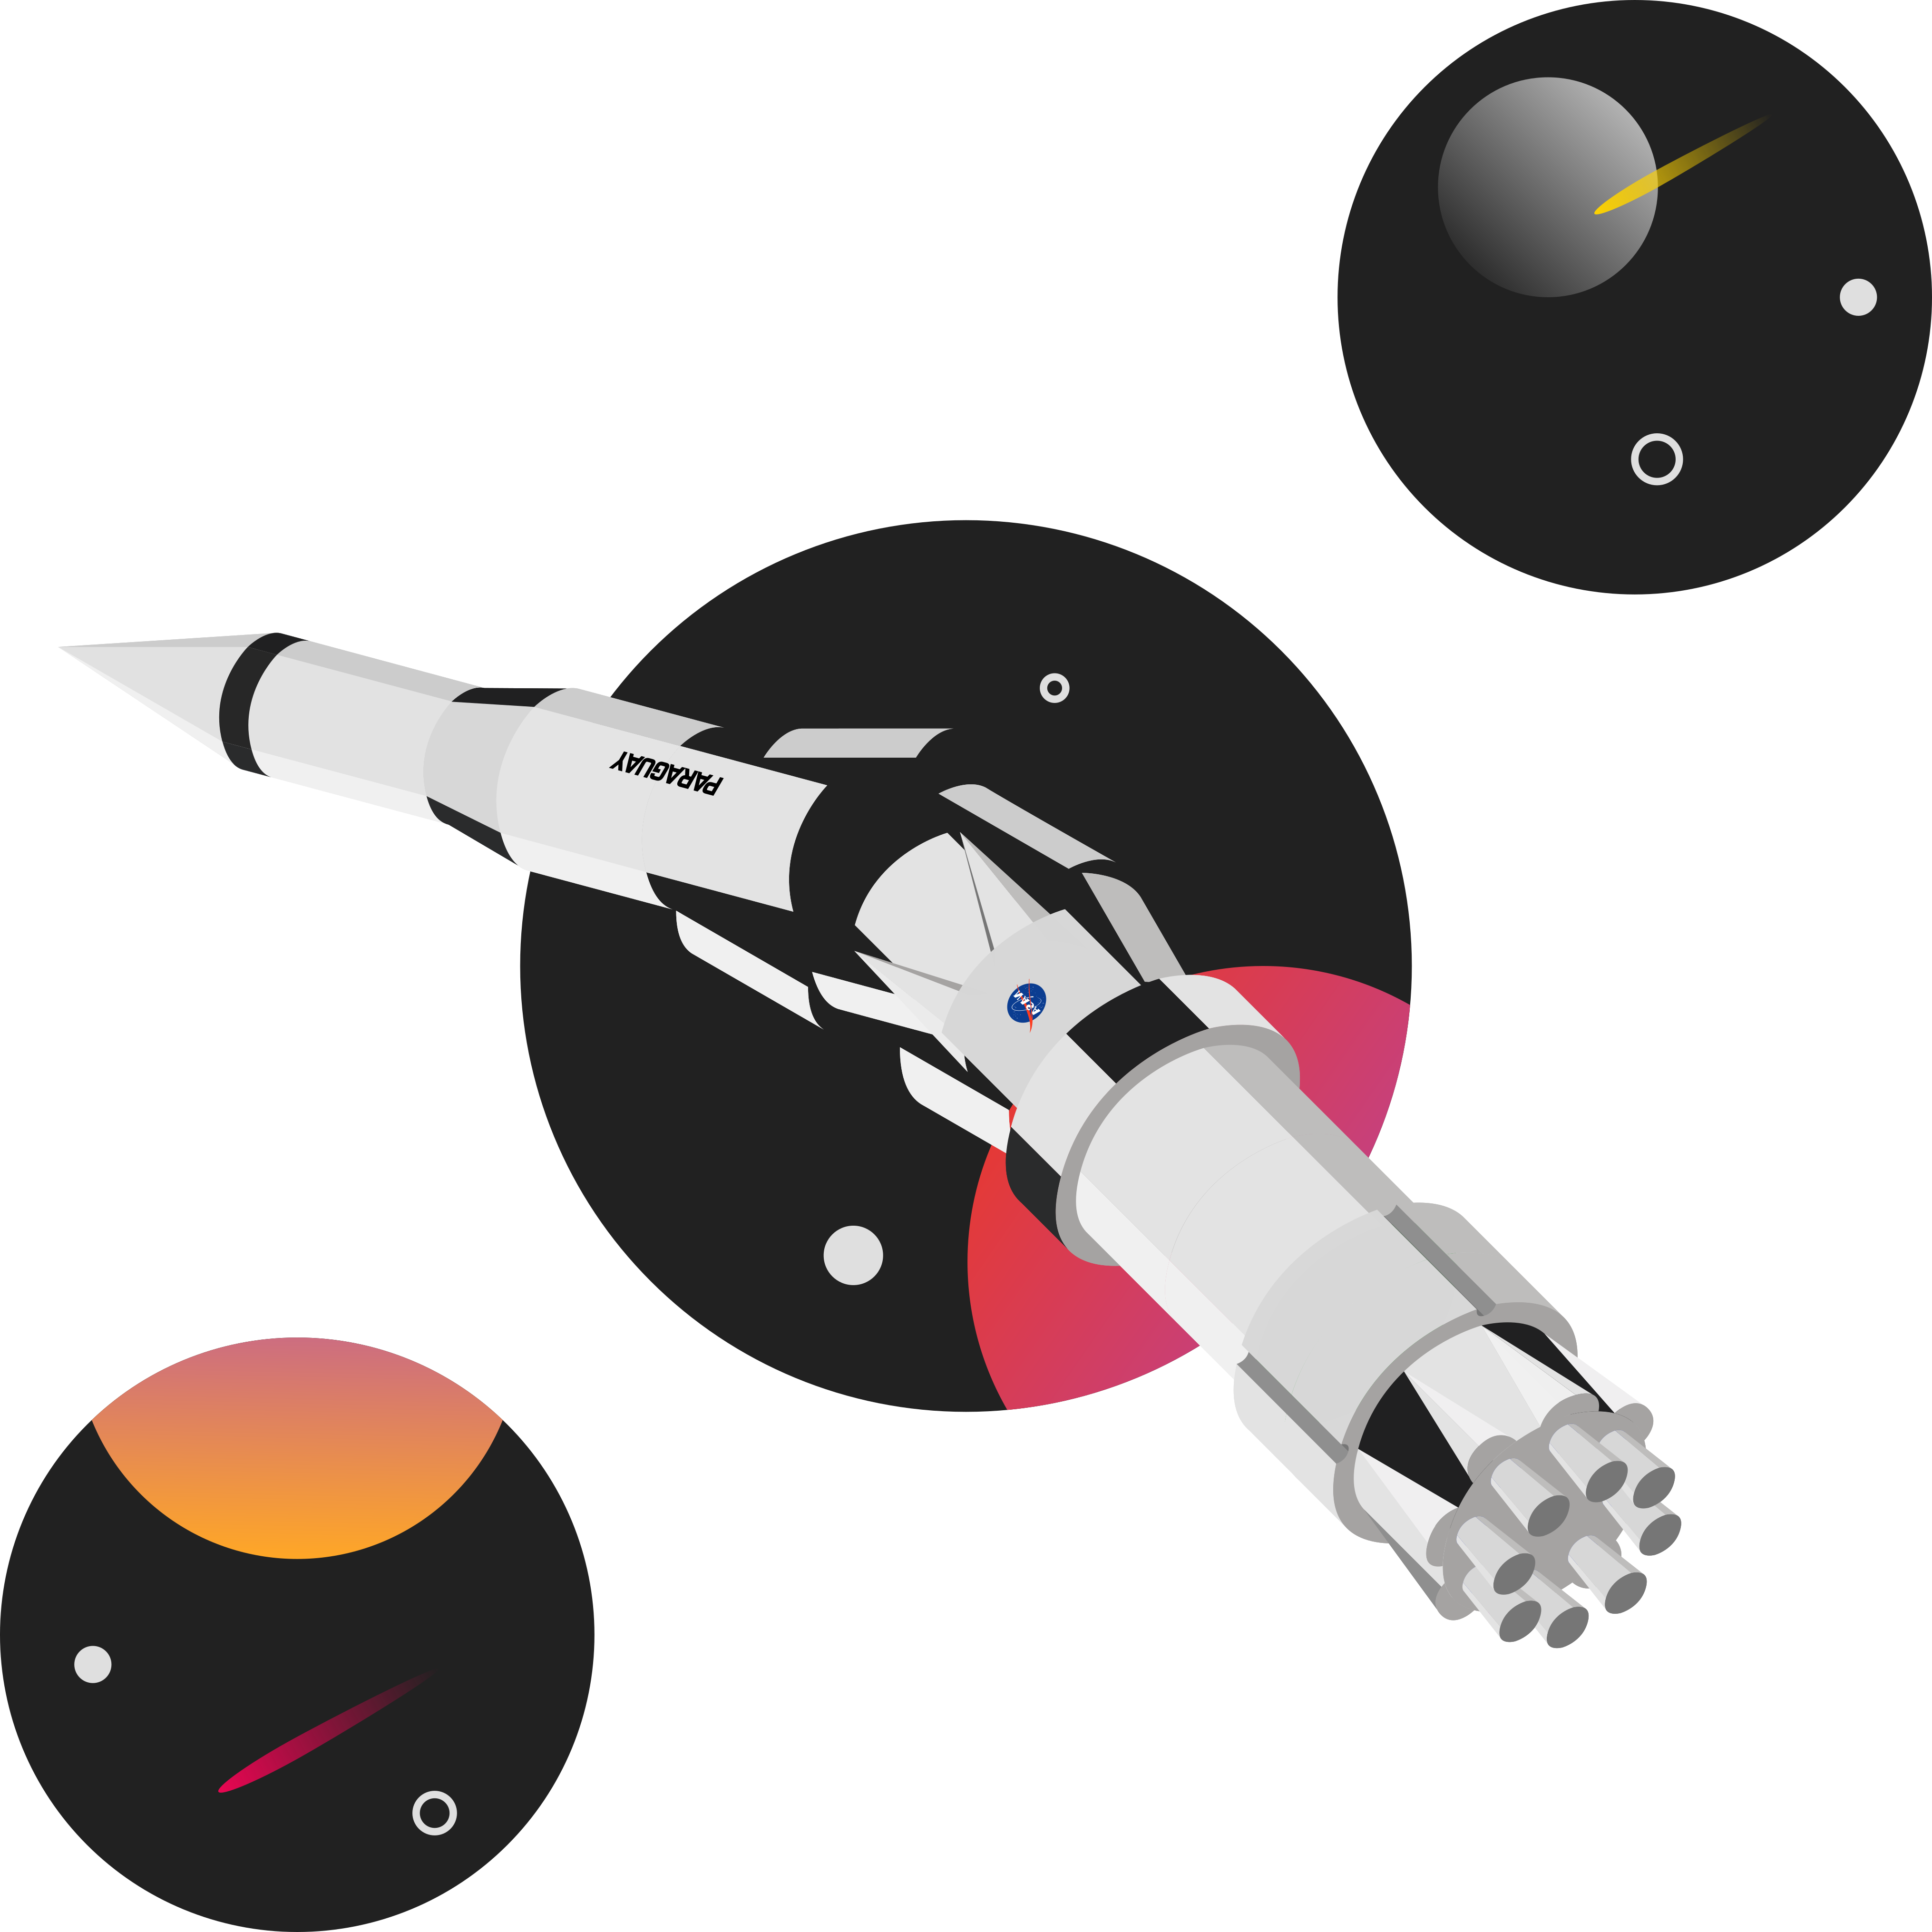
\includegraphics[scale=0.2]{images/catastrophic-failure.png}
    \caption{Praesent maximus commodo sagittis}\label{fig:test}
\end{figure}

\section{Formulas}

Lorem ipsum dolor sit amet, consectetur adipiscing elit, sed do eiusmod tempor
incididunt ut labore et dolore magna aliqua. Ut enim ad minim veniam, quis nostrud
exercitation ullamco laboris nisi ut aliquip ex ea commodo consequat. Duis aute
irure dolor in reprehenderit in voluptate velit esse cillum dolore eu fugiat nulla
pariatur. Excepteur sint occaecat cupidatat non proident, sunt in culpa qui officia
deserunt mollit anim id est laborum.

\begin{align}
    \int_a^b f(x) \diff x &= \evalat{F(x)}{a}{b} \\
                          &= F(b) - F(a)           
\end{align}

\newpage

\medskip
\printbibliography

\end{document}
